\chapter{Styles: The Menu}\label{ch:bibstyles}

\indexstart{styles!overview}
There are many different citation and bibliography styles available
for \biblatex, and half the battle is finding one which meets your
needs as closely as possible. But before looking at them in detail,
it's a good idea to try to identify them broadly.

\tikzstyle{level 1}=[level distance=2.5cm, sibling distance=2cm]
\tikzstyle{level 2}=[level distance=2.5cm, sibling distance=2cm]
\tikzstyle{level 3}=[level distance=2.5cm, sibling distance=1cm]
\tikzstyle{bag}=[text width=4em, text centered]
\tikzstyle{end}=[circle, minimum width=3pt, fill, inner sep=0pt]

\begin{figure}
\sffamily
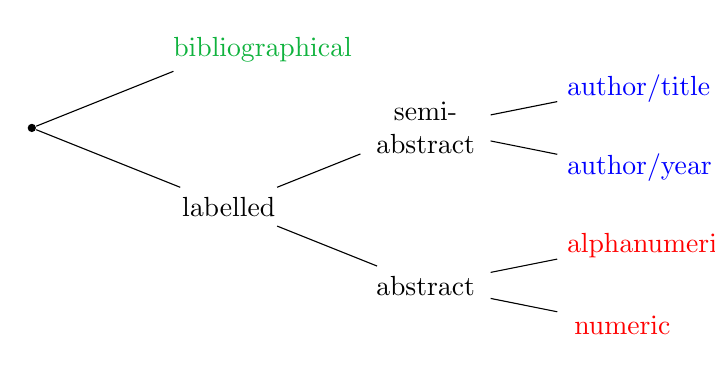
\begin{tikzpicture}[grow=right]
\node[end]{}
  child {
    node[bag] {labelled}
        child {
           node[bag] {abstract} 
              child {
           node[bag, color=red]{numeric}}
              child {
           node[bag, color=red]{alphanumeric}
           }
          }
        child  {
           node[bag] {semi-abstract}
              child  {
                node[bag, color=blue]{author/year} }
              child  {
                node[bag, color=blue]{author/title}}
         }}
  child {
    node[bag,color=red!20!blue!30!green] {bibliographical}
  };
\end{tikzpicture}
\caption{Citation: Family Tree}
\end{figure}

The first big division is between styles which rely on \emph{labels}
and those that place full bibliographical information directly into
citations. In labelled styles the bibliography contains the essential
information about a citation, and the text contains references which
are not self-contained, but are intended to allow the reader to
cross-refer to the bibliography. In contrast, in unlabelled styles,
bibliographical information can be found in the citations
themselves. It may be repeated in the bibliography. But the reader is
not expected to need to look anything up in the bibliography to find
information about the work cited. However, because this consumes so
much space, it is common to find a system of cross-references and
abbreviations (including, in extreme cases, a panoply of latin
gadgets: ibid., op.\ cit., loc.\ cit., supra, infra).

The next division is between \emph{abstract} labelling systems and
\emph{partly meaningful} labelling systems. In an abstract labelling
system, the label carries no bibliographical information at all.
It might be simply a number. To follow it up, the reader
\emph{must} look it up in the bibliography. In a partly meaningful
labelling system (typically an author/year system), the label does
provide some information which is likely to mean something:
it tells you who wrote the work, and when. But the information is
still not comprehensive, and the reader who wanted to track down the
specific source would still need to use the bibliography.

\begin{table*}[tbh]
\setfloatalignment{t}
\caption[][-5cm]{Examples of citations in different families}
\begin{tabular}{lp{6cm}p{6cm}}
\toprule
& \textsf{first citation} & \textsf{later citations} \\
\cmidrule(lr){2-2}\cmidrule(lr){3-3}
\textsf{bibliographic} & M.\ Nussbaum, \emph{Poetic Justice} (Beacon
Press: Boston, 1995) & Nussbaum, op.\ cit.\ supra n. \emph{x}\\
& & ibid. \\
\textsf{author/title} & Nussbaum, \emph{Poetic Justice} & Nussbaum,
\emph{Poetic Justice}\\
\textsf{author/year} & (Nussbaum 1995) & (Nussbaum 1995) \\
\textsf{alphabetic label} & [Nus85] & [Nus85]\\
\textsf{numeric} & [1] & [1] \\
\bottomrule
\end{tabular}
\end{table*}

Of course, within each family there is considerable
variation. Numerical systems\marginnote{[1] (1) $^1$ [1, 5--8, 10] [1,
  8, 10, 7, 6, 5]} may place numbers in brackets, or parentheses, or
as superscript; they may sort and compress ranges, or leave them
uncompressed; they may sort the bibliography alphabetically and then
put references in, or they may present the bibliography in the order
in which the works happen to appear in the text. \marginnote{(Author
  1980) (Author: 1980) (Author, 1980)}Author/year systems may format
their references in a variety of different ways. And
full-bibliographical systems differ tremendously\marginnote{supra
  n. $\theta$, n $\theta$ above, (n $\theta$)} in the range of latin
gadgets they regard as acceptable or necessary. But these differences,
though important, are less pronounced than the fundamental differences
between the types of citation.  \indexstop{styles!overview}

\package{Biblatex} styles also fall into these three families, and
there are a number of `standard' styles in each. In principle,
\biblatex\ distinguishes between the `citation
style'\marginnote{\cs{usepackage[citestyle=...]\{biblatex\}}} (which
determines how citations appear in the text) and the `bibliography
style'\marginnote{\cs{usepackage[bibstyle=...]\{biblatex\}}} (which
determines how the list of references is printed; it is possible to
specify each separately. In practice, however, there tends to be a
connection between these things, and most users will not specify them
separately, but will simply specify a \verb|style| option when loading
\biblatex\, which will load both citation style and bibliography
style. That is what we assume here.

Another line of division within \biblatex\ styles is between generic
styles and specific styles. Generic styles (like the standard
\biblatex\ styles) reflect common citation practices but do not insist
on conforming to any particular style guide. Specific styles aim to
provide accurate implementations of particular detailed guides. In
principle, there is much to be said for specific styles, which are
more likely to be accurate reflections of citation practices in the
field to which they relate.

\indexstart{bibliography style!specific styles}
If you are looking for a \biblatex\ style the first question should be
whether there is an existing style which aims to implement the
particular citation style you are following. There are many such
packages available on \smallcaps{ctan} (a selection is given in table
\ref{ctan:bespoke}). However, you do need to be careful, because while
some of the packages---for instance \package{biblatex-apa} and
\package{biblatex-chicago}---are very stable and solidly maintained,
others are less polished and mature. The only solution is to test.

\index{bibliography style!APA}\index{bibliography style!AIP}%
\index{bibliography style!APS}\index{bibliography style!American Chemical Society}%
\index{bibliography style!Angewandte  Chemie}%
\index{bibliography style!Historische Zeitschrift}\index{bibliography style!Chicago}%
\index{bibliography style!IEEE}\index{bibliography style!MLA}%
\index{bibliography style!Nature@\emph{Nature}}%
\index{bibliography style!NEJM}%
\index{bibliography style!Royal Society of  Chemistry}%
\index{bibliography style!Science@\textit{Science}}%
\index{bibliography style!OSCOLA}%
\index{bibliography style!philosophy}%
\index{bibliography style!SBL}%
\begin{table}
\caption{Packages for Particular Styles\label{ctan:bespoke}}
\small
\begin{tabular}{llll}
\toprule
\textsf{style}                            & \textsf{package}                 & \textsf{version} & \textsf{date} \\
\midrule AIP                     & \texttt{biblatex-phys}           & 1.0b             & 2016          \\
APA                              & \texttt{biblatex-apa}            & 7.4              & 2017          \\
APS                              & \texttt{biblatex-phys}           & 1.0b             & 2016          \\
American Chemical Society        & \texttt{biblatex-chem}           & 1.1s             & 2017          \\
Angewandte Chemie                & \texttt{biblatex-chem}           & 1.1s             & 2017          \\
\textit{Historische Zeitschrift} & \texttt{historische-zeitschrift} & 1.1a             & 2014          \\
Chicago                          & \texttt{biblatex-chicago}        & 1.0rc1           & 2016          \\
IEEE                             & \texttt{biblatex-ieee}           & 1.2a             & 2017          \\
MLA                              & \texttt{biblatex-mla}            & 1.9              & 2016          \\
\textit{Nature}                  & \texttt{biblatex-nature}         & 1.3b             & 2017          \\
NEJM                             & \texttt{biblatex-nejm}           & 0.4              & 2011          \\
Royal Society of Chemistry       & \texttt{biblatex-chem}           & 1.1s             & 2017          \\
\textit{Science}                 & \texttt{biblatex-science}        & 1.1g             & 2016          \\
OSCOLA                           & \texttt{oscola}                  & 1.5              & 2017          \\
Philosophy                       & \texttt{biblatex-philosophy}     & 1.9              & 2017          \\
SBL                              & \texttt{biblatex-sbl}            & 0.8.1            & 2017          \\  
\bottomrule
\end{tabular}
\end{table}

\indexstop{bibliography style!specific styles}\index{bibliography style!general styles}

The second type of style is not tied to any concrete style guide or
set of rules, but aims to reflect general academic practice and to
provide a reasonable style which can be used or
adapted.\marginnote{See, in particular, the \texttt{biblatex-dw}
  styles.} The standard styles that come with \biblatex\ are in this
category. But there are also other styles, available on
\smallcaps{ctan} which are also like this. These styles often aim at
providing a large amount of configurability and
flexibility.\index{bibliography
  style!biblatex-dw@\texttt{biblatex-dw}}

\index{bibliography styles!choosing a style}
So how should you choose a style? The ideal situation is that the
exact style you want already exists. There's a good chance that is the
case. For instance, in the humanities, the Chicago styles (which offer
both an author/year and a full bibliographical form) are very commonly
used; and between the APA style (which is an author/year style), the
MLA style (which is an author/title style) and the various styles for
scientific journals, you may well find you are covered. If so, use
that style (and consult its documentation carefully). Scientists are
also well covered by a variety of different numeric styles. A variety
have been illustrated with examples at the end of this
document.\intref{See page~\pageref{chapter:examples}} The \biblatex\
documentation also includes many examples, together with the document
that produced them.

If there isn't an exact style that is precisely what you want, you
will have to find one that comes close to your needs, and either live
with it or adapt it. Provided your requirements are not rigidly
fixed,\footnote[][-3ex]{If requirements \emph{are} absolutely
  rigid, it sometimes turns out to be impossible to meet them
  precisely without adaptations that are not easy to make. Generally,
  if the adaptation requires re-ordering the information that is
  printed, it is likely to be fairly hard to do, whereas if it
  requires simple re-styling, it should be quite simple.} you can
probably find something which is satisfactory.

I'm not going to say much more of the precisely tailored styles:
you'll know if those are what you want. The rest of this chapter
surveys some of the standard (and a few of the other available
`general' styles) to help you understand what they provide. It's
helpful to consider them family-by-family. But bear in mind that
the main strength and purpose of \biblatex\ is not in its in-built
styles, which are intended rather as starting points for adjustment
than as a bibliographic \emph{dernier cri}. Still, much of what is
said about them is generally applicable.

\indexstart{bibliography style!numeric!standard}
\subsection{Standard Numeric Styles}

Numeric styles, though rather tedious to produce in the days of
typewriters and hot metal type, are quite convenient for computers,
and we will start with those. There's really room for variation in
four areas:
\begin{itemize}
\item Whether the references are listed in order of (first) citation,
  or sorted into a logical order (usually, alphabetical by name of
  author).
\item Exactly how the bibliographical entries are formatted internally
  (for instance whether journal articles are printed in italics, or
  put in quotation marks).
\item The precise format of references in the text. Numbers, of
  course: but are they in brackets [1] or parentheses (1) or
  superscript$^{1}$? Are they perhaps in bold \textbf{[1]}. If there
  are multiple citations are they separated by commas [1, 2]; or
  perhaps by semi-colons [1]; [2]?
\item How to handle ranges. If I cite items 1, 3, 4, 8, and 5, should
  I end up with the citation [1, 3, 4, 8, 5], or should it be sorted
  [1, 3, 4, 5, 8], or should it be sorted and compressed [1, 3--5, 8]?
\end{itemize}

How do the \biblatex\ standard numeric styles deal with these issues?

\index{bibliography style!numeric!bibliography format}
It's easiest to deal with the actual formatting of the bibliographical
material first, because that doesn't change: all the numeric styles handle it
in the same way. Figure \ref{numeric-examples} shows two very ordinary
book and article references, formatted as the standard styles do.

\begin{figure}
\fbox{\includegraphics{./examples/cotton-numericu.pdf}}
\caption{Numeric bibliography style\label{numeric-examples}}
\end{figure}

If that doesn't look right for you, you will need either to try to
identify an existing numeric bibliography style which is correct, or
to adapt the standard in some way.

\index{bibliography style!numeric!sorting citations}\index{bibliography style!numeric!compressing citations}
\newthought{Sorting is the next thing} to consider. In \biblatex\ that
is dealt with by a package option which specifies the sorting method
to be used. If you are used to \package{bibtex} this will be
unfamiliar to you, because traditionally \package{bibtex} `baked in'
the sorting mechanism to the bibliography style.

By default, the numeric styles in \biblatex\ sort the references into
alphabetical order: looking first at the name of the author or editor,
then at the title, and then at the year. If you want citations to be
listed in \emph{citation order}, you will need to specify the option
\begin{center}
\verb|sorting=none|
\end{center}
when you load \biblatex.\intref{See chapter~\ref{ch:sorting} for much
  more information on sorting.}

\begin{margintable}[4cm]
\begin{tabular}{lll}
\toprule
                       & \textsf{numeric} & \parbox{6ex}{\textsf{numeric-comp}} \\
\midrule\cs{cite\{a\}} & [1]              & [1]                                 \\
\cs{cite\{a,b\}}       & [1, 2]           & [1, 2]                              \\
\cs{cite\{b,a\}}       & [2, 1]           & [1, 2]                              \\
\cs{cite\{a,b,c\}}     & [1, 2, 3]        & [1--3]                              \\
\cs{cite\{c,a,b\}}     & [3, 1, 2]        & [1--3]                              \\
\bottomrule
\end{tabular}
\vspace{3pt}
\caption{Effect of compressing and sorting}
\end{margintable}
\newthought{That takes us to the form and order of references}, and at
this point the standard styles do offer some options, particularly in
terms of order.
\begin{enumerate}
\item If you want references \emph{uncompressed} and \emph{not
    reordered}, just load the style \verb|numeric|. The package will
  then print the references you give in any citation in exactly the
  order you cited them in.
\item If you want references \emph{sorted and re-ordered} but
  \emph{not} compressed, then load the style \verb|numeric|, but also
  add the option |sortcites=true|. (This, at least, you will surely
  nearly always want!)
\item If you want references \emph{sorted and compressed}, then load
  the style \verb|numeric-comp|
\end{enumerate}
(There's also a style called
  \texttt{numeric-verb}. It's described at in the \biblatex\
  documentation; but it's rather rarely useful.)

\index{bibliography style!numeric!superscript}
When it comes to changing the citation format, the most common
requirements can be met as follows For \emph{superscript citations},
you have three options:
\begin{enumerate}
\item Use the \cs{supercite}
  command\marginnote{\texttt{blah.}\cs{supercite\{a\}}
    $\rightarrow$blah.$^{1}$} instead of \cs{cite}: this will produce
  superscript citations.
\item Load \biblatex\ with the option \verb|autocite=superscript| and
  then use the \cs{autocite} citation command instead of \cs{cite}.
\item Remap \cs{cite} to \cs{supercite} (or to \cs{autocite} with the
  \verb|superscript| option set).
\end{enumerate}

\index{bibliography style!numeric!punctuation}
Changing the \emph{punctuation between multiple citations} is easy. By
default it's a comma. You change it by redefining
\cs{multicitedelim}.\intref{See further, chapter \ref{ch:recipes}} So
if you want a semicolon, you would put (in your preamble)
\begin{center}
\verb|\renewcommand{\multicitedelim}{\addsemicolon\space}|
\end{center}

Occasionally one sees styles where the label is in bold or some other
funny font. If you have to do that, you need to provide field formats
for \verb|labelprefix|, \verb|labelnumber| and
\verb|entrysetcount|. Each takes the same form (in the preamble of
your document, assuming you wanted bold):
\begin{center}
\verb|\DeclareFieldFormat{labelnumber}{\textbf{#1}}|
\end{center}
Or whatever other format you want.

If you want to use \emph{parentheses} instead of brackets around
citation labels ---so you get (1) instead of [1]---or if you want to
dispense with these delimiters altogether, you need to do rather more
work. This topic is covered in some detail below.\intref{p~\pageref{recipe:brackets}}
\indexstop{bibliography styles!numeric!standard}
\indexstart{bibliography styles!alphanumeric!standard}
\section{Alphanumeric Labels}

Alphanumeric labels look like [JW86] or [Jon95]. They are a half-way
house between the elegant simplicity of numerical citations, and the
additional information provided by author/year styles.

If you need or want to use such a system, load either the style
\verb|alphabetic| or \verb|alphabetic-verb|. The only difference
between the styles is how multiple citations are treated: with
\verb|alphabetic| you get them enclosed in a single set of
brackets\marginnote{\cs{cite\{a, b\}}\gives [AA01, BB02]} separated by
commas whereas with \verb|alphabetic-verb| you get each reference in
its own set of brackets, separated by
semicolons.\marginnote{\cs{cite\{a, b\}}\gives [AA01]; [BB02]}

The printed bibliography is obviously essential to a style that uses
alphanumeric labels, because the reader has to have a way of looking
up what the labels mean. The bibliography will look something like
figure \ref{example:bibliography:alphabetic}

\begin{figure}
\caption{A bibliography with alphanumeric
  labels\label{example:bibliography:alphabetic}}
\fbox{\includegraphics{./examples/cotton-alphabeticu.pdf}}
\end{figure}

\index{bibliography styles!alphanumeric!citation sorting}
\newthought{Compression obviously makes no sense} for labels (how
would one do it?) but you can, if you like have them sorted by setting
the option \verb|sortcites=true|: they will be placed in the same
order they appear in the bibliography. But you may be interested in
how the label actually gets constructed.

If you don't like the labels that \biblatex\ produces in a particular
case, you can override its decision in one of two ways.

\index{bibliography style!alphanumeric!custom labels}
First, if the \verb|shorthand| field is set, then \biblatex\ will use
it instead of the label. So, for instance, if we set
\begin{verbatim}
@book{book1,
  author = {Author, A.},
  date   = {1989},
  ...
  shorthand = {Masterpiece},
}
\end{verbatim}
then \verb|\cite{book1}| will produce [Masterpiece], not [AA89].

Alternatively, you can directly set the \verb|label| field. In
practical terms, that will produce the same result.
\begin{verbatim}
@book{book1,
  author = {Author, A.} 
  ...
  label = {MyLabel}
}
\end{verbatim}
and \verb|\cite{book1}| produces [MyLabel89]. You can see the difference:
whereas the \verb|shorthand| field is used `as is', the \verb|label|
field substitutes only the alphabetic part of the label: the year part
is still added automatically.

A still more advanced change would be to alter altogether the way that
labels are generated. This is an advanced customization, which is not
covered in this document: consult the \biblatex\
documentation.\intref{\emph{Manual} \S\ 4.5.4}

\index{bibliography style!alphanumeric!punctuation}
\newthought{In terms of formatting} there's not much room for
variation.
\begin{itemize}
\item You can change the punctuation that gets printed between
  multiple sources (by default, a comma in \verb|alphabetic| and a
  semicolon in \verb|alphabetic-verb|) by redefining
  \cs{multicitedelim}.
\item You can alter the font in which the label gets printed: you will
  need to alter the field format for both \verb|labelalpha| and
  \verb|extraalpha|. So, for instance, for bold labels you want
\begin{quote}
\verb|\DeclareFieldFormat{labelalpha}{\mkbibbold{#1}}|\\
\verb|\DeclareFieldFormat{extraalpha}{\mkbibbold{#1}}|
\end{quote}
\end{itemize}
\index{bibliography style!alphanumeric!standard}

\section{Author/Year Styles}

Author/year styles set citations in a form such as (Bloggs 1982). They
are common in many humanities subjects. Where an author has more
than one work in the same year, alphabetic labels are added to make it
clear which work is which (Bloggs 1982a, Bloggs 1982b). Labels are
usually placed directly in the text, not in footnotes. The
bibliography is necessary in order to provide detailed
bibliographical information that is lacking in the text: it is usually
organised to as to put author and year first in each entry, where it
can easily be found.

\begin{figure}
\caption{Author/year bibliography\label{example:bibliography:authoryear}}
\fbox{\includegraphics{./examples/cotton-authoryearu.pdf}}
\end{figure}

\indexstart{bibliography style!author/year!standard} The standard
\biblatex\ styles offer a small selection of different author/year
citation styles. (Among the other available styles, the APA style, and
the Chicago style if loaded with the \verb|authordate|
option\footnote{The \package{Chicago} style is loaded with
  \cs{usepackage[...]\{biblatex-chicago\}} rather than
  \cs{usepackage[style=chicago]\{biblatex\}}.} provide very fully
developed author/year styles, which might well be preferable to the
standard styles for many people.)

\index{bibliography style!author/year!compressing}\index{bibliography style!author/year!ibid}
\index{ibid!author/year styles, in}
The essential questions you need to ask in order to choose a style
are:\begin{itemize}
\item Do You want citations \emph{compressed}? In other words, if you
  cite (in a single citation) two works by the same author, do you
  want to see `Doe 1982; Doe 1983' (uncompressed) or `Doe 1982, 1983'
  (compressed).
\begin{margintable}
\begin{tabular}{lll}
\toprule
                          & \textsf{compress} & \textsf{ibid} \\
\midrule
\texttt{authoryear} \\
\texttt{authoryear-comp}  & \textbullet \\
\texttt{authoryear-ibid}  &             & \textbullet \\
\texttt{authoryear-icomp} & \textbullet & \textbullet \\
\bottomrule
\end{tabular}
\vspace{3pt}
\caption{Author/Year styles\label{authoryear:styles}}
\end{margintable}
\item Do you want to use `ibid' for repeated citations of the same
  source? (In other words, should successive citations of a given work
  produce `(Bloggs 1982) \ldots\ (ibid., p.~100)' instead of `(Bloggs
  1982) \ldots\ (Blogs 1982, p.~100)'. 
\end{itemize}
Depending on the answer to those questions, load the appropriate style
as shown in table \ref{authoryear:styles}. (If you want multiple
citations sorted but not compressed, you can set the option
\verb|sortcites| while loading an uncompressed style.)

\newthought{Besides selecting} from the range of styles, there's not
much room for simple customization; but there are three things you may
wish to adjust.

\index{bibliography style!author/year!names}
First, the number of names that get printed.\intref{See further, p~\pageref{recipes:maxnames}}  By default, up to three names will be
printed, both in the citations and in the bibliography. If there are
more than three names, they will be abbreviated to one name `et al'
--- again, both in the citations and the bibliography. So, for
instance, the entry:
\begin{Verbatim}
@book{companion,
  author = {Goossens, Michel and Mittelbach, Frank 
            and Samarin, Alexander},
  title = {The LaTeX Companion},
  date  = {1994},
  ...
}
\end{Verbatim}
will produce `Goosens, Mittelbach, and Samarin 1994'; but if one
additional author were added, the citation would become `Goosens et
al'.

This behaviour can be altered,\intref{For further detail, see
  p~\pageref{recipes:maxnames}} and it can be altered separately for
references in the text and those in the bibliography list. If you
prefer shorter lists of names, then use the option \verb|maxnames|: if
\verb|maxnames=1| then no more than one name will be used, and so
forth. You can, however, still have more than one name in the
bibliography, because you can set \verb|maxbibnames| to a different
number. So if, for instance, \verb|maxnames=1| but
\verb|maxbibnames=3|, then the in-text citations will read `Goosens et
al', but the bibliography will still read `Goosens, Mittelbach, and
Samarin \ldots'.

\index{bibliography style!author/year!punctuation}
A second adjustment you might want to make is to
punctuation:\intref{See generally, chapter \ref{ch:recipes}.}
\begin{itemize}
\item You might change the punctuation between author and the year. By
  default it is a space; one way to change it is by renewing the
  \verb|\nameyeardelim|.\intref{For more information about delimiters,
    and some more complex ways of handling them, see \emph{Manual},
    \S~3.10.2} For instance, if you wanted to place a colon, rather
  than a comma, you would
\begin{verbatim}
\renewcommand{\nameyeardelim}{\addcolon\space}
\end{verbatim}
  and citations would become `Author: 1980', and so forth. Another way
  of changing it uses the command
  \cs{DeclareDelimFormat}\manref{3.10.2}. So the same result is
  achived with\label{declaredelim}
\begin{verbatim}
\DeclareDelimFormat{nameyeardelim}{\addcolon\space}
\end{verbatim}
  Note that if you used the |\DeclareDelimFormat| method, the name of
  the delimiter is not preceded by a backslash.
\item You can change the punctuation between multiple citations, by
  changing \verb|\multicitedelim|, either using |\renewcommand| or
  using |\DeclareDelimFormat|.
\end{itemize}

\index{bibliography style!author/year!ibid}\index{ibid!ibidtracker option@\texttt{ibidtracker} option}
\label{citations:ibid}
The third set of adjustments that you might like to make arise only if
you are using one of the style versions that makes use of `ibid'. You
can control the circumstances in which ibid is used by setting the
\verb|ibidtracker| option.\label{ibidtracking} There are five possible
settings for \verb|ibidtracker| described in the \biblatex\
documentation; but in my experience only three of them are useful
\begin{description}[font=\ttfamily\upshape]
\item[ibidtracker=false] Don't ever use ibid.
\item[ibidtracker=constrict] Use ibid, but be cautious to avoid
  ambiguity. Footnotes and the main text are tracked separately, and
  ibid is used only if the reference will certainly be unambiguous.
\item[ibidtracker=true] The sloppiest use of ibid: use ibid whenever
  the previous reference was to the work in question, without tracking
  text and footnotes separately.
\end{description}
In most cases, the use of any setting sloppier than \texttt{constrict}
seems questionable (and this is the default setting).
\indexstop{bibliography style!author/year!standard}

\indexstart{bibliography style!author/title!standard}
\section{Author/Title Styles}

The various author/title styles all use the author's name as the
primary citation label. Depending on the particular style, a title is
either always added, or is added only where it seems necessary to
disambiguate the citation (because more than one work is being cited
by the same author). A bibliography remains essential to the style,
and will look like figure
\ref{example:bibliography:authortitle}. However, the author/title
styles lurk especially close the the borderline between labelled and
fully bibliographical styles, and are appropriate for use either in
footnotes or in running text. (In fact, the default styles which come
with \biblatex\ differ as to whether they place citations generated
with the \cs{autocite} command in text or footnotes.)

\begin{figure}
\caption{Author/title bibliography\label{example:bibliography:authortitle}}
\fbox{\includegraphics{./examples/cotton-authortitleu.pdf}}
\end{figure}

Simple as this may seem, there are actually a large number of standard
styles dealing with this. They can however, be selected by answering
three questions:

\index{bibliography style!author/title!sorting citations}
\index{bibliography style!author/title!compressing citations}
\begin{enumerate}
\item Do you want citations \emph{sorted and compressed}. Suppose you
  have two works by Joseph Bloggs, his \emph{First Book} and his
  \emph{Second Book}, and one by John Smith, his \emph{Book}. If you
  \verb|\cite{bloggs1,smith,bloggs2}| an uncompressed style will give
  you `Bloggs, \emph{First Book}; Smith, \emph{Book}; Bloogs,
  \emph{Second Book}'. A compressed style will give you `Bloggs,
  \emph{First Book}, \emph{Second Book}; Smith, \emph{Book}'.
\item \index{bibliography style!author/title!terse forms}Do you want
  citations to be \emph{terse}. If you use terse citations, then
  titles will be included only if they are required in order uniquely
  to identify the source. So, in the above example, titles will be
  included for Bloggs (because you are citing two works by him), but
  not for Smith, because you are citing only one. So
  \cs{cite}\texttt{\{bloggs1, bloggs2, smith\}} will give you `Bloggs,
  \emph{First Book}; Bloggs, \emph{Second Book}; Smith'.
\item \index{bibliography style!author/title!ibid}\index{ibid!author/title styles}If you
  cite the same work successively, do you want to use `ibid'. If you
  do, then
\begin{quote}
\ttfamily
Some \verb|\parencite{smith}}| have pointed out that this is an unnecessarily
complex range of options \verb|\parencite[100]{smith}|.
\end{quote}
will give you 
\begin{quote}
Some (Smith, \emph{Book}) have pointed out that this is an
unnecessarily complex range of options (ibid, p.~100).
\end{quote}
\begin{margintable}
\begin{tabular}{lccc}
\toprule
                            & \textsf{compress} & \textsf{terse} & \textsf{ibid} \\
\midrule \textsf{authortitle}                                                    \\
\texttt{authortitle-comp}   & \textbullet                                        \\
\texttt{authortitle-terse}  &                   & \textbullet                    \\
\texttt{authortitle-ibid}   &                   &                & \textbullet   \\
\texttt{authortitle-icomp}  & \textbullet       &                & \textbullet   \\
\texttt{authortitle-tcomp}  & \textbullet       & \textbullet                    \\
\texttt{authortitle-ticomp} & \textbullet       & \textbullet    & \textbullet   \\
\bottomrule
\end{tabular}
\vspace{3pt}
\caption{Author/title styles\label{authortitle:styles}}
\end{margintable}
\end{enumerate}

Based on the answer to these questions, you can choose from among the
various author/title styles that are available. See table
\ref{authortitle:styles}.\footnote{The one missing style seems to be
  the combination of terse citations with ibid.} (If you want multiple
citations sorted but not compressed, you can use an uncompressed style
but set the \verb|sortcites| option.)

\newthought{Customization} is not often required, but resembles that
for the author/year styles.\intref{And see chapter \ref{ch:recipes}.}
\begin{itemize}
\item \index{bibliography style!author/title!names} Customization of
  the number of names printed in citations and the bibliography is
  achieved using \verb|maxnames| and \verb|maxbibnames|, just as
  described above.
\item \index{bibliography style!author/title!punctuation} The separator
  between author and title is usually a comma. To change it, redefine
  \cs{nametitledelim}. For instance, to change it to a colon,
\begin{verbatim}
\renewcommand{\nametitledelim}{\addcolon\space}
\end{verbatim}
\item The delimiter between multiple citations is usually a
  semicolon. To change it, redefine \cs{multicitedelim}.
\item If you are using ibid,\intref{Page \pageref{ibidtracking}.} you
  can configure it using the options given above.
\end{itemize}
\indexstop{bibliography style!author/title!standard}

\index{bibliography style!author/title!authortitle-dw@\texttt{authortitle-dw}}
\newthought{Apart from the standard styles} that come with \biblatex,
there is a very sophisticated, and highly configurable, style written
by Dominik Waßenhoven, the \texttt{authortitle-dw} style, which is
part of the \package{biblatex-dw} style package.

\section{Verbose styles}

\indexstart{bibliography style!verbose!standard}
The essence of verbose or bibliographical citation styles is that they
include information which is strictly bibliographical in the citations
themselves. Because of this, they are principally designed to be used
in footnotes --- the information the provide would clutter text up
much too much. And, quite often, in order to avoid excessive
repetition of the same data, these styles make use of a variety of
abbreviations or shorthands, such as \emph{ibid.}, \emph{op.\ cit.},
\emph{loc.\ cit.}, \emph{supra} and so on, though exactly which of
these are used and how varies quite a bit from style to style.

Because these styles place the full bibliographical data in the text,
the bibliography is more of an adjunct than an essential reference
tool. (It actually looks, in the standard styles, just like the
author/title bibliography in figure
\ref{example:bibliography:authortitle}.)

\index{bibliography style!verbose!Chicago}\index{bibliography style!verbose!footnote-dw@\texttt{footnote-dw}}
Standard\marginnote{The standard verbose styles are, I think, not
  especially usable as they stand; but they form an excellent starting
  point for customization.} \biblatex\ offers no fewer than seven
different flavours of verbose citation style. For practical use, there
should be added to these the \verb|footnote-dw| style from Dominik
Waßenhoven's \package{biblatex-dw} bundle, the
\package{biblatex-chicago} package, with option \verb|notes| and the
\package{oscola} style --- all of which build on the standard styles
to handle quite complex citations. In many cases these may be found
more convenient, though the standard styles are definitely the right
place to start if you are looking to produce a custom style of your
own.

As in the author/year and author/title styles, the essential choice
from the menu of verbose styles can be made by asking a few simple
questions.
\begin{enumerate}
\item How do you want to handle repeat citations. The first time you
  cite a source, all the verbose styles will give you a full
  citation. The second time, all will give you a shortened
  citation. But do you want that shortened citation to be simply a
  short name? Or do you want a cross-reference added to the note in
  which the source was first cited?
\item Do you want to use \emph{ibid} where two immediately sequential
  citations are to the same source?
\item Do you want to use additional scholarly abbreviations such as
  \emph{op cit} and \emph{loc cit}?
\end{enumerate}

\begin{table*}[btp]
\small
\begin{tabular}{lp{1.7in}p{1.7in}p{1.7in}}
\toprule
                                               & \textsf{first citation} & \textsf{subsequent} & 
\textsf{repeated}                                      \\
\midrule verbose                               & Frank Albert Cotton et al. \emph{Advanced inorganic
  chemistry}. 6th ed. Chichester: Wiley, 1999  & Cotton et al.,
\emph{Advanced inorganic chemistry}            & Cotton et al., \emph{Advanced
  inorganic chemistry}                                 \\
verbose-ibid                                   & Frank Albert Cotton et al. \emph{Advanced inorganic
  chemistry}. 6th ed. Chichester: Wiley, 1999  & Cotton et al.,
\emph{Advanced inorganic chemistry}            & Ibid. \\
verbose-note                                   & Frank Albert Cotton et al. \emph{Advanced inorganic
  chemistry}. 6th ed. Chichester: Wiley, 1999  & Cotton et al.,
\emph{Advanced inorganic chemistry}, see n. ?? & Cotton et al.,
\emph{Advanced inorganic chemistry}, see n. ??         \\
verbose-inote                                  & Frank Albert Cotton et al. \emph{Advanced inorganic
  chemistry}. 6th ed. Chichester: Wiley, 1999  & Cotton et al.,
\emph{Advanced inorganic chemistry}, see n. ?? & Ibid. \\
verbose-trad1                                  & Frank Albert Cotton et al. \emph{Advanced inorganic
  chemistry}. 6th ed. Chichester: Wiley, 1999  & Cotton et al.,
op.\ cit.                                      & Ibid. \\
verbose-trad2                                  & Frank Albert Cotton et al. \emph{Advanced inorganic
  chemistry}. 6th ed. Chichester: Wiley, 1999  & Cotton et al.,
\emph{Advanced inorganic chemistry},
op.\ cit.                                      & Ibid. \\
\bottomrule
\end{tabular}
\caption[][1em]{Various verbose styles.\label{bibliography:examples:verbose}}
\end{table*}

\newthought{Once that choice has been made} there is little scope for
customization. Or rather, there is such \emph{vast} scope for
customization of ever aspect of the citation --- much of which
requires customization of actual bibliography drivers --- that it lies
well outside the ambit of this chapter.

\index{ibid!in verbose styles}\index{bibliography style!verbose!ibid}
However there are some options which can be adjusted: the behaviour of
\verb|ibid| (see above),\intref{p~\pageref{citations:ibid}} for
example, or sorting schemes (see chapter \ref{ch:sorting}).
\indexstop{bibliography style!verbose!standard}


%%% Local Variables:
%%% coding: utf-8
%%% mode: LaTeX
%%% TeX-master: "biblatex-tutorial"
%%% End:
